\problemname{Bergskedja}
Markus blir ofta uttråkad på mattelektionerna, och har därför börjat rita olika landskap i sitt räkneblock. Han har till exempel upptäckt följande procedur för att enkelt rita en snygg bergskedja:

\begin{enumerate}
\item Börja med att rita ut marken som en horisontell linje.
\item Välj sedan ut ett antal punkter ovanför marken. Dessa punkter kommer representera bergstoppar.
\item Från varje punkt drar man sedan två linjer som skär marken i 45 graders vinkel, vilket skapar ett antal likbenta rätvinkliga triangelar.
\item Fyll sedan i trianglarna. Notera att trianglarna kan överlappa, och att man då inte behöver fylla i alla helt.
\end{enumerate}

\noindent Givet $N$ punkter som ritats ut ovanför marken, beräkna arean som behöver fyllas i för att skapa bergskedjan.

\section*{Input}
Den första raden innehåller talet $N$. De följande $N$ raderna innehåller vardera två heltal $X$ och $Y$, separerade med mellanslag. Dessa beskriver koordinaterna för de punkter som ritats ut.

\section*{Output}
Ditt program ska skriva ut ett tal på en rad, den totala arean som behöver fyllas i.

\section*{Förklaring av exempel}

\begin{figure}[ht!]
\centering
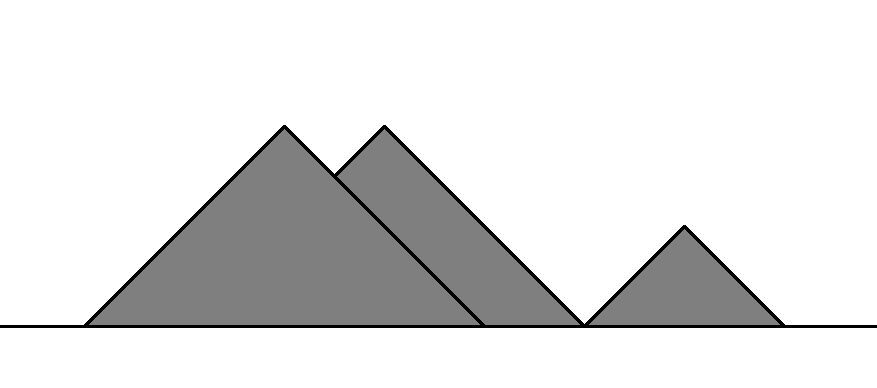
\includegraphics[width=0.7\textwidth]{bergskedja.png}
\caption{En illustration av det första exemplet.}
\label{overflow}
\end{figure}

% TODO: beskriv med text?

\section*{Poängsättning}
Din lösning kommer att testas på en mängd testfallsgrupper. För att få poäng för en grupp
så måste du klara alla testfall i gruppen.

\begin{tabular}{| l | l | l | l |}
\hline
Grupp & Poängvärde & Gränser \\ \hline
1     & 20         &  $1 \le N \le 100, -100 \le X \le 100, 0 \le Y \le 100$ \\ \hline
2     & 20         &  $1 \le N \le 100\,000, -1\,000 \le X \le 1\,000, 0 \le Y \le 1\,000$ \\ \hline
3     & 60         &  $1 \le N\le 100\,000, -100\,000 \le X \le 100\,000, 0 \le Y \le 10\,000$\\ \hline
\end{tabular}

\section*{Precision}
Ett svar på det här problemet kommer att räknas som korrekt om det absoluta felet är mindre än $10^{-3}$. Notera att man för full poäng behöver kunna skriva ut svar med många siffrors precision (se exempel 3). Om man till exempel kör C++ och cout så kommer man därför behöva ange vilken precision man vill ha innan man skriver ut svaret.

